\chapter{Introduction}

The NASA Ames Stereo Pipeline (ASP) is a suite of automated geodesy \&
stereogrammetry tools designed for processing planetary imagery
captured from orbiting and landed robotic explorers on other planets.
It was designed to process stereo imagery captured by NASA spacecraft
and produce cartographic products including digital elevation models
(DEMs), ortho-projected imagery, and 3D models.  These data products
are suitable for science analysis, mission planning, and public
outreach.

\begin{figure}[tb] 
   \centering
   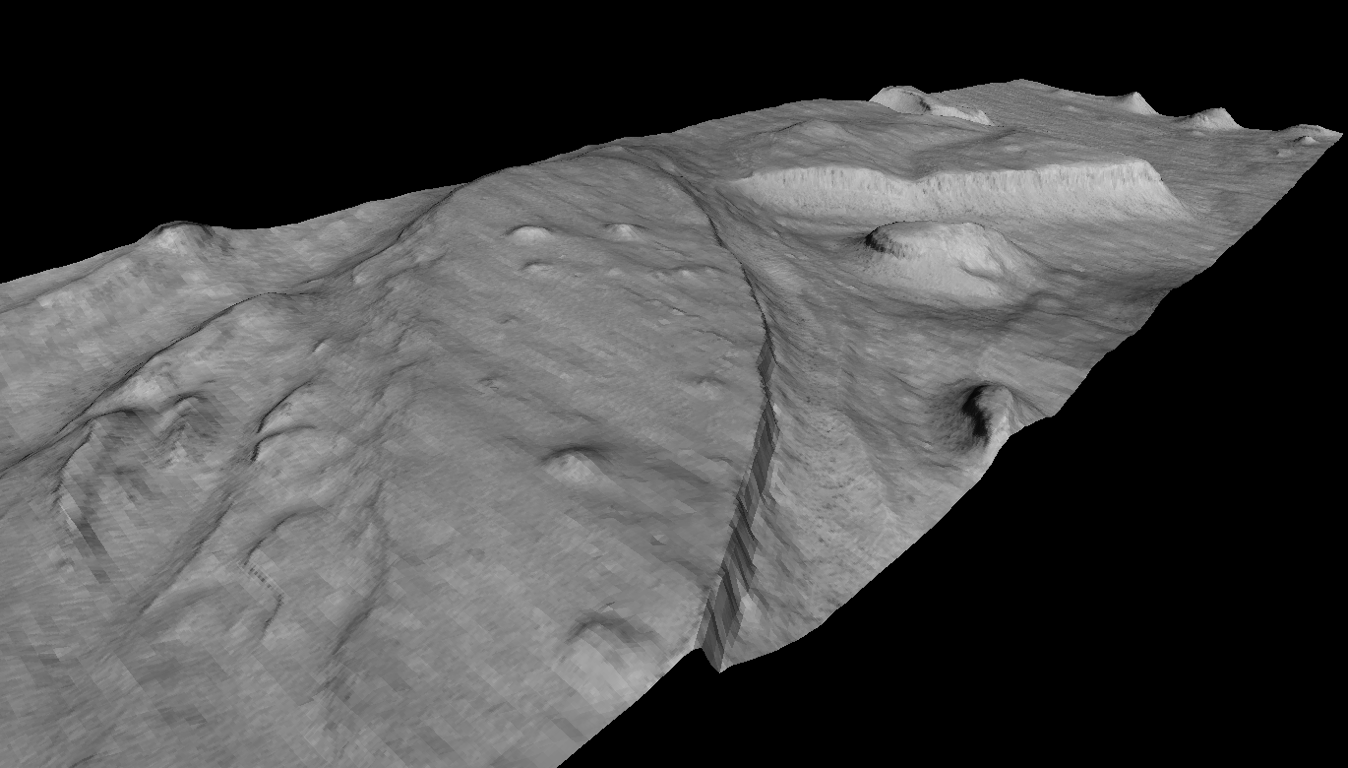
\includegraphics[width=6.5in]{images/introduction/p19view2.png} 
   \caption{This 3D model was generated from Mars Orbiter Camra image
     pair M01-00115 and E02-01461 (34.66N, 141.29E).  The complete
     stereo reconstruction process takes approximately five minutes on
     a 3.0GHz workstation for input images of this size (1024x8064
     pixels).  This model, shown here without vertical elevation
     exaggeration, is roughly 2-km wide in the cross-track
     dimension. }
   \label{fig:p19}
\end{figure}

\section{Background}

The Intelligent Robotics Group (IRG) at the NASA Ames Research Center
has been developing 3D surface reconstruction and visualization
capabilities for planetary exploration for more than a decade.  First
demonstrated during the Mars Pathfinder Mission, the IRG has delivered
tools providing these capabilities to the science operations teams of
the Mars Polar Lander mission, the Mars Exploration Rover mission, and
most recently the Mars Reconaissance Orbiter Mission. A critical
component technology enabling this work is the Ames Stereo Pipeline.
ASP generates high quality, dense, texture-mapped 3D surface models
from stereo image pairs.

Although initially developed for ground control and scientific
visualization applications, the ASP has evolved in recent years to
address orbital stereogrammetry and cartographic applications.  In
particular, long-range mission planning requires detailed knowledge of
planetary topography, and high resolution topography is often derived
from stereo pairs captured from orbit.  Orbital mapping satellites are
sent as precursors to planetary bodies in advance of landers and
rovers.  They return a wealth of imagery and other data that helps
mission planners and scientist identify areas worthy of more detailed
study. Topographic information often plays a central role in this
planning and analysis process.

Laser range-finding instruments such as the Mars Orbital Laser
Altimeter (MOLA) \citep{1992JGR....97.7781Z,2001JGR...10623689S}
has significantly advanced the study of the Martian surface by
providing geologists with a highly accurate elevation map of the
entire planet.  The upcoming Lunar Orbital Laser Altimeter (LOLA)
\citep{2008AGUFM.P31B1419N,2007SSRv..129..391C} will achieve similar
results for the Moon.  However, MOLA topographic products are limited
in resolution (463~m/pixel at the equator).  This, coupled with
localized interpolation artifacts in some regions due to sparse
laser data, have rendered MOLA products insufficient for detailed
studies of specific sites; e.g. geologic stratification and deposition
analysis, or in the case of mission planning, landing site selection.

The most common technique for obtaining higher-resolution digital
terrain models (DTMs) is to employ stereogrammetric techniques.
However, existing processing techniques on photogrammetric
workstations are extremely human intensive and expensive.  The
substantial number of man-hours and resources required for this
aproach has meant that relatively few of the existing stereo image
pairs have been processed, hence very few of these data products have
reached the scientific community.

The ASP was designed to address this shortfall by automating the
stereo reconstruction process so that it can run without human
guidance.  By applying recent advances in robotics and computer
vision, we have created an automated process that is capable of
generating high quality DEMs with minimal human intervention.  Users
of the Stereo Pipeline can expect to spend some time picking a handful
of settings when they first start processing a new type of imagery,
but once this is done the Stereo Pipeline can be used to process tens,
hundreds, or even thousands of stereo pairs without further
adjustment.


\section{Operation with the USGS Integrated Software for Imagers and Spectrometers}

This version of the Stereo Pipeline functions as an add-on for an
existing installation of the USGS Integrated Software for Imagers and
Spectrometers (ISIS).  ISIS is widely used in the planetary science
community for processing raw spacecraft imagery into high level data
products of scientific interest such as map projected and mosaicked
imagery \cite{2004LPI....35.2039A, 1997LPI....28..387G, ISIS_website}.

The Stereo Pipeline provides an advanced stereo image processing
capability for ISIS.  It supports the ISIS ``cube'' file fromat, and
can make use of the ISIS camera models and ancillary information
(i.e. SPICE kernels) for imagers on many NASA spacecraft.  This tight
integration with ISIS allows scientists to prepare data and perform
stereo porcessing using the familiar ISIS toolchain.  Another benefit
is that new sensor models are available in the ASP as soon as they are
developed for ISIS.  In principal, by leveraging the wealth of
different camera models in ISIS, stereo processing can even be carried
out with images captured by different spacecraft.  Finally, and
perhaps most importantly, the use of a single standardized set of
camera models also ensures consistency between products generated in
the Stereo Pipeline and those generated by ISIS.

The Stereo Pipeline can process arbitrary, non-ISIS images with
accompanying camera information, but doing so requires a significant
amount of extra work and setup.  This use is not covered in this
document, however feel free to contact us if you are interested in
learning more about the software's advanced capabilities.

\section{Terminology}

DISPARTY

TRIANGULATION

CORRELATION

BUNDLE ADQJUSTMENT

\section{Getting Help}

All bugs, feature requests, and general discussion should be sent to
the Ames Stereo Pipeline user mailing list:
\begin{quote}
\indent \url{stereo-pipeline@lists.nasa.gov}
\end{quote}
To subscribe to this list, send an empty email message with the
subject 'subscribe' (without the quotes) to:
\begin{quote}
\indent \url{stereo-pipeline-request.lists.nasa.gov}
\end{quote}
To contact the lead developers and project manager directly, send mail
to:
\begin{quote}
\indent \url{stereo-pipeline-owner@lists.nasa.gov}
\end{quote}

\section{Warnings to users of the Ames Stereo Pipeline ALPHA}

This is an {\bf ALPHA} release of the Stereo Pipeline.  There are many
known bugs and incomplete features. The API and command line options
will almost certainly change prior to the final release.  Some of the
documentation is incomplete and some of it may be out of date or
incorrect.  Although we hope you will find this release helpful, you
use it at your own risk.

While we are confident that the algorithms used by this software are
robust, they have not been systematically tested or rigorously
compared to other methods in the peer-reviewed literature. We have a
number of efforts underway to carefully compare Stereo
Pipeline-generated data products to those produced by established
processes, and we will publish those results as they become available.
In the meantime, {\bf we strongly recommend that you consult us before
  publishing any results based on the cartographic products produced
  by this software}. You have been warned!



